% ============================================
%  Article Class (This is a LaTeX2e document)  
% ============================================
\documentclass[12pt]{scrartcl}

\usepackage[english]{babel}
\usepackage[utf8]{inputenc}

\usepackage{enumitem}
\usepackage[round]{natbib}
\usepackage{color}

\newcommand\reft[3][]{#2~\ref{#3}#1}
\newcommand\refp[3][]{(#2~\ref{#3}#1)}
\newcommand\refsect[1]{\reft{Section}{#1}}
\newcommand\refsecp[1]{\refp{Sec.}{#1}}
\newcommand\reftabt[1]{\reft{Table}{#1}}
\newcommand\reftabp[1]{\refp{Tab.}{#1}}

% ============
%  Algorithms
% ============
\usepackage{algorithm2e}
\SetKwProg{Fn}{Function}{}{}
\newcommand\refalgt[1]{\reft{Algorithm}{#1}}
\newcommand\refalgp[1]{\refp{Alg.}{#1}}

% ======
%  Math
% ======
\usepackage{amsmath}
\usepackage{amsthm}
\usepackage{mathtools} % \mathclap
\newtheorem{thm}{Theorem}[section]
\newtheorem{cor}[thm]{Corollary}
\newtheorem{lem}[thm]{Lemma}
\newtheorem{prop}[thm]{Proposition}
\newtheorem{property}[thm]{Property}
\theoremstyle{definition}
\newtheorem{defn}[thm]{Definition}
\newtheorem{assum}[thm]{Assumption}
\theoremstyle{remark}
\newtheorem{rem}[thm]{Remarque}
\numberwithin{equation}{section}

\usepackage{amssymb}
\newcommand{\prob}[1]{\mathbb{P}\left(#1\right)}
\newcommand{\Ker}[1]{\mathrm{Ker}\left(#1\right)}
\newcommand{\Image}[1]{\mathrm{Im}\left(#1\right)}
\newcommand{\diag}[1]{\mathrm{diag}\left(#1\right)}
\newcommand{\Vect}[1]{\mathrm{Vect}\left\{#1\right\}}

% ============================
%  Figures and relative paths
% ============================
\usepackage{graphicx}
\graphicspath{{figures/}}
\usepackage{import}
\makeatletter
  \def\relativepath{\import@path}
\makeatother
\newcommand\reffigt[2][]{\reft[#1]{Figure}{#2}}
\newcommand\reffigp[2][]{\refp[#1]{Fig.}{#2}}

% ==========
%  Document
% ==========
\begin{document}

\title{Resolution of FBA}%
\author{S. Fischer - Biosys - MAIAGE}%
\date{\today}%

\maketitle

\newpage

\tableofcontents

\newpage

\section{Mathematical interpretation of FBA problems}

We consider the following mathematical problem:
\[
\left\lbrace
\begin{array}{l}
  \max c^T\nu \\
  S\nu = b \\
  \nu_i \geq 0 \textrm{ for some arbitrary $i$}
\end{array}
\right.
\]

Biologically speaking, $\nu$ is the flux vector through metabolic reactions, $b$ the exchange flux vector of metabolites with environment and other cell compartments. $S$ is the stoichiometry matrix of the metabolism. The fact that a $\nu_i\geq 0$ indicates that this specific reaction is irreversible.

\paragraph{Structure of $S$} Let $C_1$, $C_2$, ..., $C_R$ be the columns of $S$. Each column represents a metabolic reaction. Let $L_1$, $L_2$, ..., $L_M$ be the lines of $S$. Each line holds the fluxes of a specific metabolites through each reaction. Note that $R$ is the number of reactions and $M$ the number of metabolites. Generally $R > M$. Here are simple mathematical facts:
\begin{itemize}
  \item $\Image{S}=\Vect{C_1, ..., C_R}$. There is a solution if and only if $b \in \Image{S}$.
  \item $L_i^T \perp \Ker{S}$.
  \item $\Ker{S}$ contains all futile cycles. However these cycles are not necessarily possible if they contain an irreversible reaction. Because $R > M$, the dimension of the kernel is pretty high.
\end{itemize}

\paragraph{Unicity} Straightforward facts:
\begin{itemize}
  \item If there are no irreversible reactions, the solution structure is $\nu_0 + \Ker{S}$, so $\max c^T\nu = \infty$.
  \item Unicity does not depend on $b$. The idea is that $\Ker{S} \cap \{\nu_i \geq 0\}$ must be bounded in the direction pointed by $c$.
  \item Intuitively, unicity is broken if $c$ maximizes the flux of a futile cycle that is thermodynamically possible. By rewriting $S$ and/or $c$, it should always be possible to warrant unicity.
\end{itemize}

\paragraph{Properties of a unique solution} Let
\[
m = \max_{\Ker{S} \cap \{ \nu_i \geq 0 \}} c^T \nu \geq 0
\]
Suppose $m$ is reached for some $\nu^*$. Let $\lambda > 1$. $\lambda \nu^* \in \Ker{S}$ and $\lambda \nu^* \in \{\nu_i \geq 0\}$. By definition of $m$, $c^T(\lambda \nu^*) \leq m$. This leads to $\lambda m \leq m$, hence $m = 0$. This means that if there is a unique solution, it is orthogonal to $\Ker{S} \cap \{ \nu_i \geq 0 \}$. This is consistent with the view that $c$ must points in a direction where $\Ker{S} \cap \{ \nu_i \geq 0 \}$ is bounded.

\paragraph{Duality} Let us now emphasize the role of $L_i$ in association with $c$. Each line of the matrix equation reads
\[
L_i^T \nu = b_i
\]
This corresponds to a hyperplane orthogonal to $L_i$. \reffigp{fig:2D_duality}~(left) shows an example in 2 dimensions with 2 lines $L_1$ and $L_2$. The maximal value in the direction of $c$ is bounded if and only if $c$ can be expressed as linear combination of $L_1$ and $L_2$. For example, if $L_1$ and $L_2$ are colinear, there is a maximal value iff $c$ is colinear to the two vectors. If there is a third dimension, there is a maximal solution iff $c$ is coplanar with $L_1$ and $L_2$. Put shortly, there is a solution iff
\[
S^T\lambda = c
\]
has a solution.

\begin{figure}[ht]
  \centering
  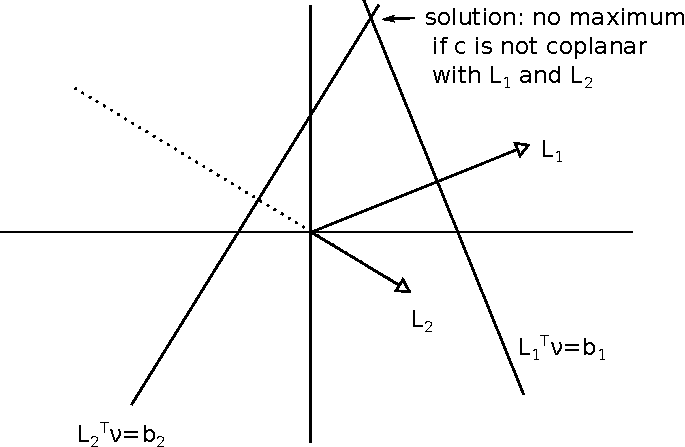
\includegraphics[width=0.4\linewidth]{2D_duality}
  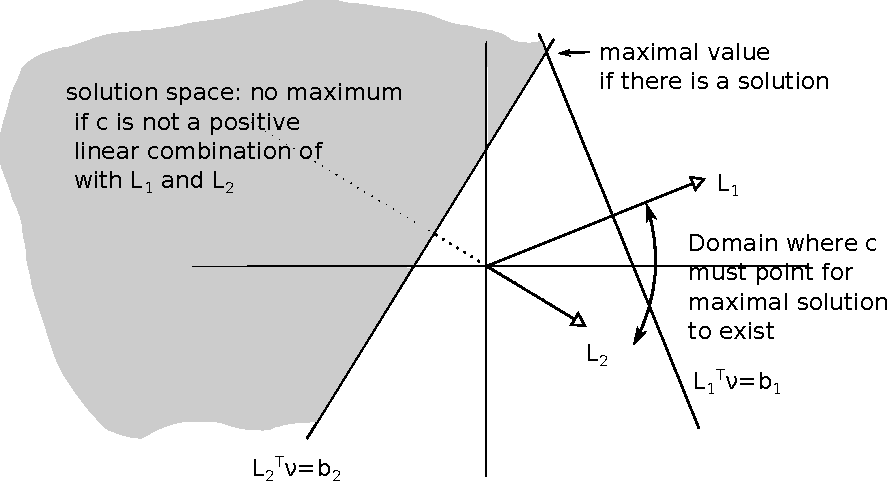
\includegraphics[width=0.55\linewidth]{2D_duality_inequalities}
  \caption{2D illustration. (Left) Solution space of $S\nu = b$. (Right) Solution space of $S\nu \leq b$.}
  \label{fig:2D_duality}
\end{figure}


\paragraph{Inequalities instead of equalities} I feel like the example above generalizes to inequalities except there is a solution iff there is a solution to
\[
S^T\lambda = c, \quad \lambda \geq 0
\]
\reffigt{fig:2D_duality}~(right) sums up this idea.

%\bibliographystyle{myplainnat}
%\bibliography{biblio}

\end{document}
% ----------------------------------------------------------------
